% 6.2 Methods
\subsection{Methods}
To demonstrate the capabilities of \textit{Segmentflow},
a full CT scan to simulation geometry workflow is demonstrated on a
mock high explosives system
consisting of F50 sand grains coated in a polymeric Kel-F binder.
The sand was coated with the binder and pressed into a cylindrical
sample. The goal of the workflow is to create segment the sand grains from
the binder and create a series of surface meshes representing each of the
tens of thousands of sand grains in the sample such that the surface mesh
representation of the sample could be loaded into a simulation software as
an initial condition for physics simulations, such as deformation.
This demonstration uses \textit{Segmentflow} to load parameters from an
input file, preprocess the CT scan images to improve the contrast, perform
a semantic segmentation to identify the sand grains, create a surface mesh
for each segmented particle and save that mesh as an STL file, and finally
postprocess the surface meshes to change the properties of the meshes.
Though this work mainly focuses on the workflow for this particular material
system and application, alternative functionality is presented throughout
the demonstration to show how the workflow and parameters might be adapted
to other systems.

\subsubsection{Input Handling}
% -------------------------------------------------------------------------
\textit{Segmentflow} was designed to create simulation-ready geometries for
a wide range of applications, so a parameter specification system is
important to tune the various algorithms the packaged leverages to segment
a specific dataset. Since \textit{Segmentflow} is a Python package, it can
easily be installed so that the functions within may be imported into other
Python scripts. However, to make \textit{Segmentflow} more user friendly,
it was structured such that it could be operated by workflow scripts. Each
script is tailored to a specific workflow and has its own accompanying input
loading function that pulls parameters from an input file in YAML format.
This allows parameters to be
listed quickly and easily with text in a human-readable way while also
listing out the potential parameters that can be adjusted without having
to dig through documentation to know what can be changed. The YAML file
format has the added benefit of allowing parameters to be grouped together.
For the \textit{Segmentflow} input file, the grouping was made according
to the section of application the parameter affects.
Grouping makes tuning segmentation behavior more clear for the user
while also improving code readability because parameters loaded into
\textit{Segmentflow} are stored in
a nested dictionary according to these groups. In an effort to further improve
accessibility, any parameters in input files are able to be left
blank to set parameters to the default value.
This allows users to use \textit{Segmentflow} even if
they are unfamiliar with the parameters. Parameter specification using an input
file makes the segmentation routine reproducible because \textit{Segmentflow}
can be executed with the same input file multiple times to achieve the same
results. A copy of the input file is
also saved to the output directory specified in the input file for two
reasons: to backfill
default values that may have been filled for empty parameters and to store
a record of segmentation parameters to preserve
reproducibility in case the original input file is altered.

\subsubsection{Preprocessing}
Image preprocessing is the portion of the F50 sand segmentation procedure
involves loading the raw 3D data and performing operations to improve the
contrast. The location of the directory as well as
the image file format are specified in the input file.
With the images loaded, the
next step of the preprocessing routine is to perform a series of steps, as
specified in the input file, to improve the contrast of the images. In the
F50 sand procedure, a median filter is applied to the CT scan
to replace each voxel with the median value of the surrounding cube
of voxels, reducing localized noise while maintaining the sharpness of
edges (unlike Gaussian filtering which will blur edges).
Intensity clipping is also performed to improve contrast by taking advantage
of the full range of available intensities according to the image data type.
This is done by providing an upper and lower percentile interval in the
input file. The range used to rescale the F50 sand sample was [0, 99.9].

\subsubsection{Semantic Segmentation}
% -------------------------------------------------------------------------
In the F50 sand sample, the classes that exist within the images are
void, particle and binder.
\textit{Segmentflow}
uses an implementation of this algorithm \textit{scikit-image}.
Multi-Otsu thresholding divides an
image into \textit{N} classes based on the distribution of intensities in
an image by maximizing inter-class variance. To make \textit{Segmentflow}
more flexible, \textit{N} is included as an
input file parameter for some workflow scripts.
\textit{Segmentflow} also includes a custom thresholding algorithm that
uses a Gaussian filter to smooth the histogram of the 3D image, calculate the
local maxima corresponding to the peak intensity relating to the three
feature classes in images (void, binder, and sand grain). Minima are found
between each of the maxima and used as the threshold values
(\ref{fig/06/thresh}).

\begin{figure}[ht]
    \centering
    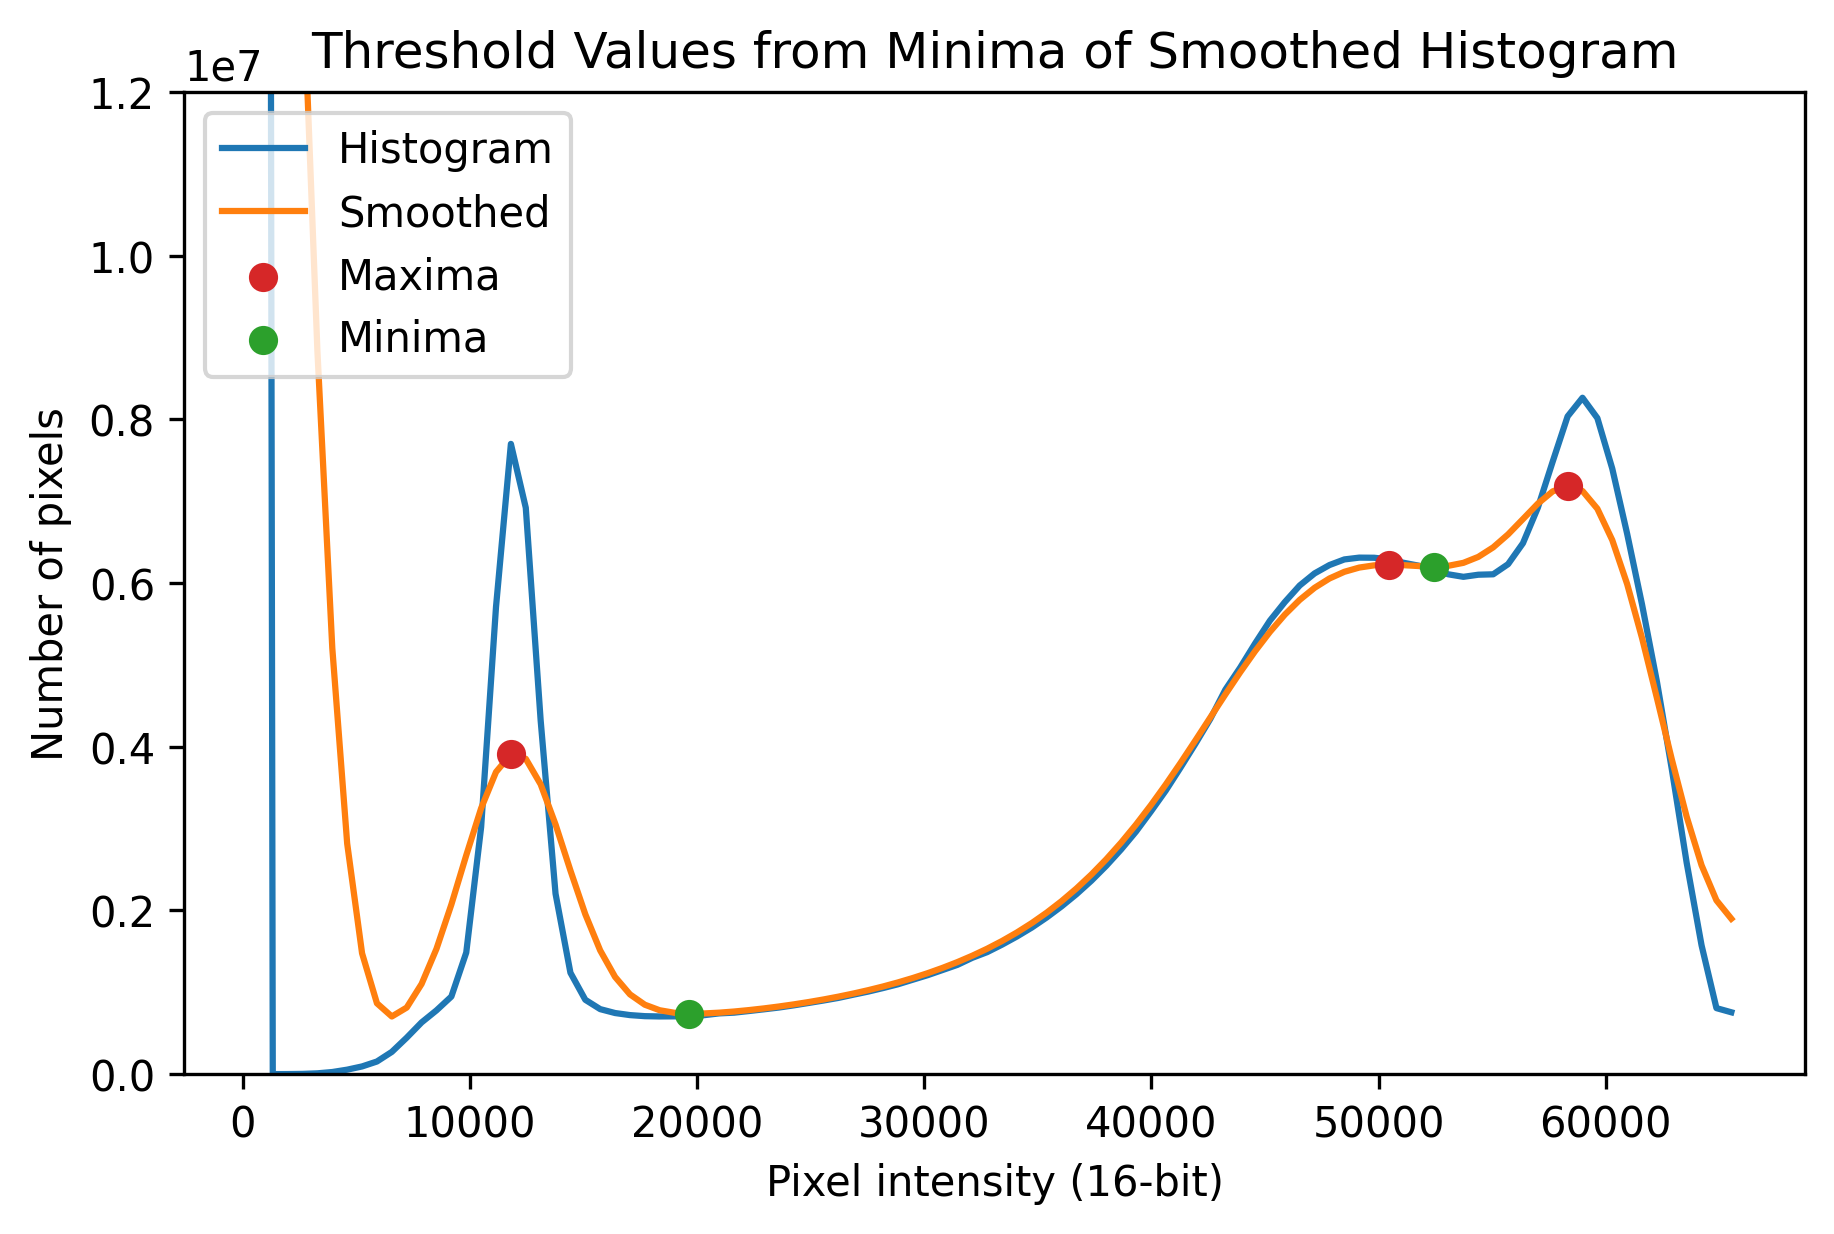
\includegraphics[width=0.75\textwidth]{figures/06/01-multi-min-hist.png}
    \caption{
        \small\setstretch{1}
        Histogram processing used to determine the threshold values to
        perform semantic segmentation on images. The blue line represents the
        raw histogram. The orange line represents the smoothed histogram.
        The red points denote the local maxima. The green points denote
        the local minima between these maxima which are used to threshold the
        material classes.
    }
    \label{fig/06/thresh}
\end{figure}

If this is a sufficient amount of segmentation
for the given application, \textit{Segmentflow}
can save a voxel representation of
the classes without undergoing further segmentation of the foreground. If
this option is specified in an input file, each voxel of a class is
represented by a unique integer label and saved as a collection of 2D
images. Otherwise, after dividing the image into \textit{N} classes, a
subset of those classes are selected to form a binary image which is used
to segment the defined class or classes into instances and/or
create surface meshes of the features. To demonstrate the instance
segmentation capabilities of \textit{Segmentflow}, the semantic
segmentation of the F50 sand sample (\ref{fig/06/semantic}.c) is
binarized by selecting only the class corresponding to the sand grains.

\begin{figure}[ht]
    \centering
    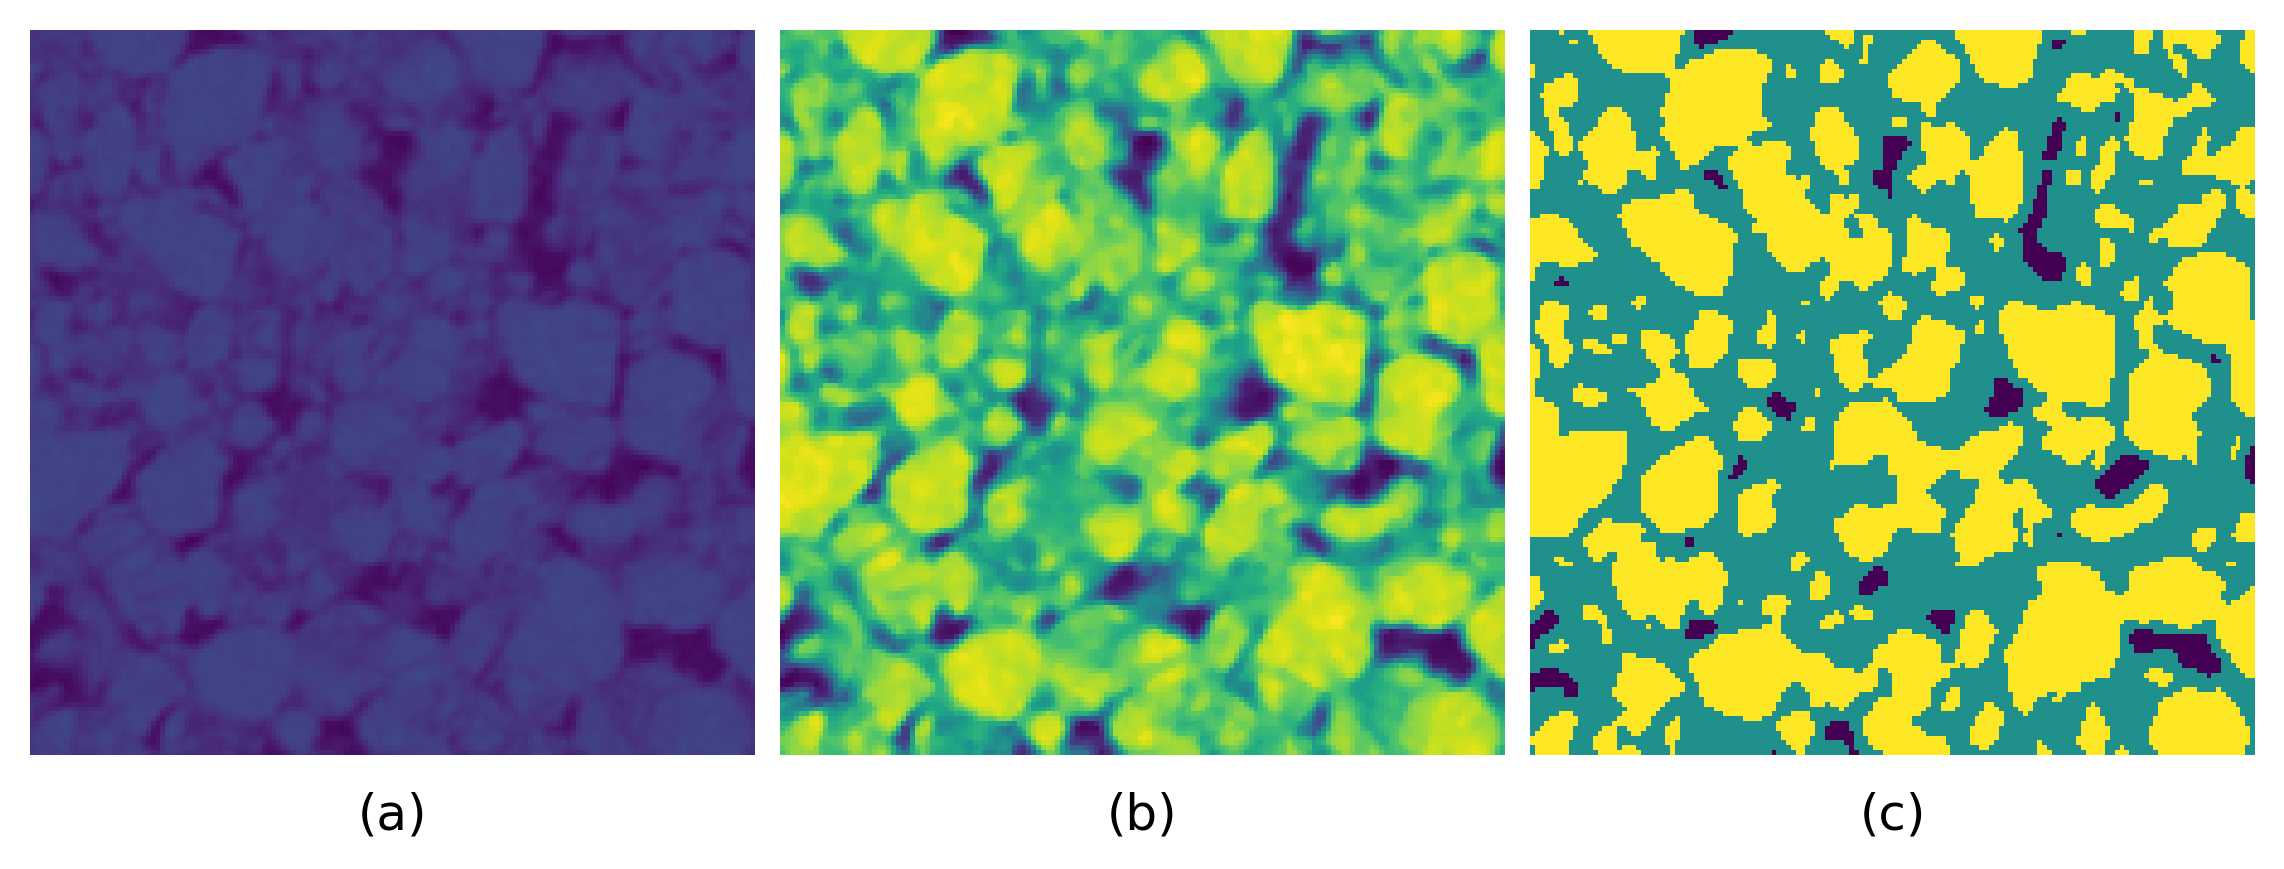
\includegraphics[width=0.75\textwidth]{figures/06/02-slice-525-semantic.png}
    \caption{
        \small\setstretch{1}
        (a) Low contrast image slice from raw CT scan.
        (b) Image slice after intensity is rescaled.
        (c) Semantic segmentation following thresholding of rescaled image
        using the minima of the smoothed histogram
        (\ref{fig/06/thresh}). The purple regions represent the
        void class, the blue regions represent the binder class, and the
        yellow regions represent the sand grain class.
    }
    \label{fig/06/semantic}
\end{figure}

\subsection{Instance Segmentation}
% -------------------------------------------------------------------------
\textit{Segmentflow}
uses a watershed algorithm in 3D to perform instance
segmentations. First a distance map is calculated by applying an EDT algorithm
implemented in \textit{scikit-image} to a binary image.
In the case of this demonstration of the F50 sand sample, a distance map
is created using the binary image corresponding to the sand grain class.
Local maxima are calculated to determine the markers which will
seed the watershed algorithm.
The 2D metaphor of watershed flooding does not
extend well to 3D, but the marker points act as the starting locations from
which the segmented regions will ``grow'' outwards.
Not all local maxima from the distance map are used as markers. Only the
maxima separated by a minimum distance are used.
The final segmentation depends greatly on
this minimum peak distance value as the number of markers is equal to the
number of labeled features, or segmented particles, in the resulting
segmentation.
If this value is too large, the results will be under-segmented as
fewer markers than sufficient are passed to the watershed algorithm,
excluding maxima that are closer together than this minimum distance.
This would create segmented particles larger than the true sand grains.
If the value is too large, the opposite will be true: too many maxima are
identified and passed to the watershed algorithm as seeds. With more markers
than necessary, the results will be over-segmented as separate markers
identified in the same feature will split that feature into multiple segmented
regions. This would produce segmented particles smaller than the true sand
grains.
Segmentations were performed at a range of minimum peak distances and
the resulting particles were analyzed to determine which minimum peak
distance value yielded particle sizes closest to typical F50 sand.

\subsubsection{Surface Mesh Creation}
% -------------------------------------------------------------------------
Depending on simulation type, a voxel representation of the segmented
particles may be an adequate format for the geometry. However,
some simulations require geometries be represented as a surface mesh
rather than voxels. Segmentflow can output triangular surface meshes saved
as STL files for each feature segmented.
There are currently two voxel preprocessing methods available in
\textit{Segmentflow} to
simplify geometries before any surface meshes are created: voxel smoothing
and morphologic erosion. For each method, the voxels of each segmented
feature are first isolated in a new 3D array. In voxel smoothing, a median
filter is applied to the voxels such that each voxel is replaced by the
median value (foreground or background) of the surrounding voxels (3 x 3 x 3
cube).
In morphologic erosion, the outer layer of voxels is removed, as if
peeling an onion. This is performed using an algorithm implemented in
\textit{scikit-image}. The algorithm can be applied multiple times
(peeling multiple onion skins) to further reduce the overall size of a
feature. This can be useful to ensure voxels of separately segmented
features are not in contact.
After these steps, surface meshes are created
for the segmented features using a marching cubes algorithm. This algorithm
takes the voxels at the surface of the 3D feature and generates
a surface consisting of vertices and triangles connecting the vertices
\cite{Lorensen1987, Lewiner2003}.
Each triangle has one of 26
possible normals based on the position of the other surface voxels in the
immediate vicinity: six possibilities for the Cartesian vectors when
neighbors of a voxel form a flat surface, 12 vectors when the voxels form
an edge, and eight vectors when voxels form a corner.
The \textit{scikit-image} implementation of the algorithm allows a voxel step
size to specified
to control the granularity of the voxels used to create the surface
mesh. If a step size of 1 is used, each voxel is analyzed to create the
surface mesh, whereas step sizes larger than 1 produce coarser mesh
results, compromising finer-scale details of the volume. Resulting surface
meshes can be saved as STL files.

\subsubsection{Surface Mesh Postprocessing}
% -------------------------------------------------------------------------
The surface meshes output from the marching cubes algorithm are blocky due
to the limited number of surface normals output from the data. This is an
artifact of the voxel nature of the data passed into the marching cubes
algorithm and is therefore not truly representative of real-world
geometries. \textit{Segmentflow} has two mesh postprocessing methods to further
process the 3D data: smoothing and mesh simplification.
Smoothing the blocky surface meshes
output by the marching cubes is achieved through Laplacian smoothing,
which interpolates normals vectors for the faces of a mesh. These meshes
may still have a large number of surface elements however because the
smoothing operation does not change the number of triangles. To reduce the
number of triangles, simplification can be performed through quadric
decimation \cite{Garland1997}. \textit{Segmentflow} implements the mesh
simplification by accepting a target number of triangles for the final
mesh and a scale factor that allows the number of triangles to be reduced
iteratively. Often smaller simplification factors yield better results
because more of a surface's shape is able to be retained between smaller
simplifications. Tuning the size of output surface meshes is an important
feature of \textit{Segmentflow} because the complexity of the meshes will
in part determine the scale of a simulation using the geometries.

